\documentclass[a4paper,12pt,french]{book}
\usepackage[margin=2cm]{geometry}
\usepackage[thinfonts,latinmath]{uglix2} 
\setcounter{chapter}{13}
\newcommand{\file}[1]{\tw{#1}}
\newcommand{\fleche}{$\blacktriangleright$\ }

\begin{document}

\chapter*{Compression de l'information}


\section{La compression en général}
	
	On peut considérer qu'un document, une image, une musique, une vidéo, un programme, ou un ensemble composé de ces éléments est une 
	\textit{information} au sens large du terme.
	Nous avons vu comment divers formats de données sont représentés en machine.
	Pour stocker ces informations ou pour les transmettre via Internet, on a tout intérêt à les \textit{compresser}.\\
	
	Compresser une information représentée par une séquence de bits $A$, c'est appliquer un algorithme qui va la transformer en une séquence B plus 
	courte que A, mais dans laquelle l'information contenue dans A subsistera, soit à l'identique, soit de manière très similaire.

	On range les algorithmes de compression en 2 catégories :
\begin{enumerate}[--]

		\item 	La \textbf{compression de données sans perte :} l'algorithme de compression est une fonction $c$ (au sens mathématique du terme) qui 
		transforme une séquence de bits $A$ en $c(A)$, telle que la longueur de $c(A)$ est inférieure à celle de $A$.\\
				La décompression est le processus inverse et est alors sans perte: on dispose d'une fonction $d$ avec la propriété suivante : quelle 
				que soit la séquence de bits $A$, $d(c(A))=A$.\\
				Autrement dit, en décompressant une séquence compressée, on obtient la séquence originale \textit{à l'identique}.
		\item 	La \textbf{compression de données avec perte : } ne s'applique qu'aux données \og perceptibles\fg{} telles que le son, l'image ou la 
		vidéo. Les données à
				 compresser peuvent parfois subir d'importantes modifications, et la perte d'information est irréversible, mais cela n'est pas ou peu 
				 perceptible par 
				 l'humain, et en tout cas, l'information abstraite contenue dans les données perceptibles reste transmise (par exemple, un fichier 
				 MP3 de très mauvaise 						qualité contenant un discours politique sera compris dans son intégralité en dépit de 
				 cette très mauvaise qualité).\\
\end{enumerate}

\begin{definition}
	On  considère un algorithme de compression qui transforme une séquence de bits $A$ (non vide) en $B$.\\
	Le \textit{taux de compression} se calcule ainsi : $1-\dfrac{\text{longueur de }B}{\text{longueur de }A}$	
\end{definition}
	
\begin{exercice}
Un algorithme d'encodage au format MP3 procède ainsi : il encode un morceau de musique de 5 minutes \og qualité CD \fg{}, c'est à dire stéréo, 16 
bits, 44 100Hz, et produit un fichier de 5 Mo.\\
Quel est le taux de compression ?
\end{exercice}

\section{Un exemple d'algorithme de compression : la compression JPEG}

	JPEG (Joint Photographic Experts Group) est un comité d'experts qui édite des normes de compression pour les images fixes. C'est aussi un format 
	de fichier d'image.
	Le format JPEG standardisé a été adopté en 1992. Il est très populaire sur Internet, on le trouve aussi dans les appareils photo et les 
	téléphones portables.\\
	
\begin{exercice}
	\begin{enumerate}[--]
		\item 	Ouvrir le fichier \file{tricoloring.png} avec GIMP (clic droit, ouvrir avec GIMP)
		\item 	Exporter ce fichier en format .jpg (CTRL+E). Activer l'aperçu dans une fenêtre d'image, faire varier le curseur de qualité et 
		observer l'aperçu. Zoomer si nécessaire (CTRL + molette souris).\\
		Qu'observe-t-on ? \`A quelle catégorie l'algorithme de compression JPEG appartient-il ?

		\item 	Régler la qualité sur 70\%, puis sauvegarder le résultat.\\
				Comparer les tailles des fichiers (dans l'explorateur Windows, faire : clic droit > propriétés) et calculer le taux de compression à 
				$10^{-2}$ près.\\
	\end{enumerate}
\end{exercice}

\section{Un algorithme de compression sans perte simple : RLE}

Le  \textit{run-length encoding}, appelé en français le codage par plages, est sans doute de l'algorithme le plus simple auquel on puisse penser. 
Voici un exemple avec des mots :
\begin{enumerate}[--]
	\item 	\tw{aaaaaaaabbbbbbbbbbbbcccccccccc} devient \tw{a8b12c10} (ici on y gagne).
	\item 	\tw{abcdef} devient \tw{a1b1c1d1e1f1} (ici on y perd).
\end{enumerate}

\begin{exercice}
Pour une image, l'encodage RLE consiste à indiquer pour chaque suite de pixels d'une même couleur le nombre de pixels de cette séquence.\\

Vous allez travailler avec le fichier \file{rle.py}. Celui-ci utilise le module \tw{image}, que nous avons déjà utilisé par le passé.\\

Coder la fonction \tw{compresse} qui compresse une image suivant ce modèle :
\begin{enumerate}[--]
	\item 	La fonction crée une liste. Les deux premiers éléments sont la largeur et la hauteur de l'image.
	\item 	Les éléments suivants vont 2 par deux : une liste de 3 éléments correspondant à une couleur de pixel, puis le nombre de fois que ce pixel 
	se répète.
			Exemple : \tw{[255,0,128],36}
	\item 	Tester la fonction sur le fichier \file{gamut.ppm}.\\
			Quelle est la taille, en \pythoninline{int} de l'image de départ ?
			Quelle est la taille, en \pythoninline{int} de la liste correspondant à l'image compressée ?
			Calculer le taux de compression.\\
	\item 	Recommencer avec le fichier \file{doudouchat.ppm}.\\
			Comment expliquer de tellles différences de taux ?
\end{enumerate}
\end{exercice}

\section{Un algorithme performant : le codage de Huffman}

	C'est un algorithme de compression sans perte. 
	Il est utilisé lors de la compression JPEG, en conjonction avec d'autres méthodes qui, elles, entrainent des pertes d'information.
	Il a inspiré les algorithmes de compression actuels, tel gzip, le logiciel libre de compression le plus utilisé actuellement.\\
	
	Compressons le texte \og this is an example of a huffman tree\fg : 
	on commence par compter les occurences de chaque lettre du texte :
	\begin{center}
	\begin{tabular}{|c|c|c|c|c|c|c|c|c|c|c|c|c|c|c|c|}
	\hline 
	o & u & x & p & r & l & n & t & m & i & h & s & f & e & a & espace \\ 
	\hline 
	1 & 1 & 1 & 1 & 1 & 1 & 2 & 2 & 2 & 2 & 2 & 2 & 3 & 4 & 4 & 7 \\ 
	\hline 
	\end{tabular}
	\end{center}
	
	
	\double{ 	Puis on va créer un arbre dont les feuilles seront les lettres du texte.\\
	 			Dans chaque n\oe ud on stockera un poids et éventuellement une lettre.\\
	 			On commence par créer les feuilles, puis on regroupe deux par deux les n\oe uds de poids minimal, en un n\oe ud dont le poids est 
	 			égal à la somme de ces deux poids.\\
	 			On répète le processus jusqu'à ce qu'il ne reste plus qu'un n\oe ud.\\
	 			Pour finir, on choisit arbitrairement d'affecter $0$ à \og droite \fg{} et $1$ à \og gauche \fg{} (ou bien le contraire).
	 			}{ 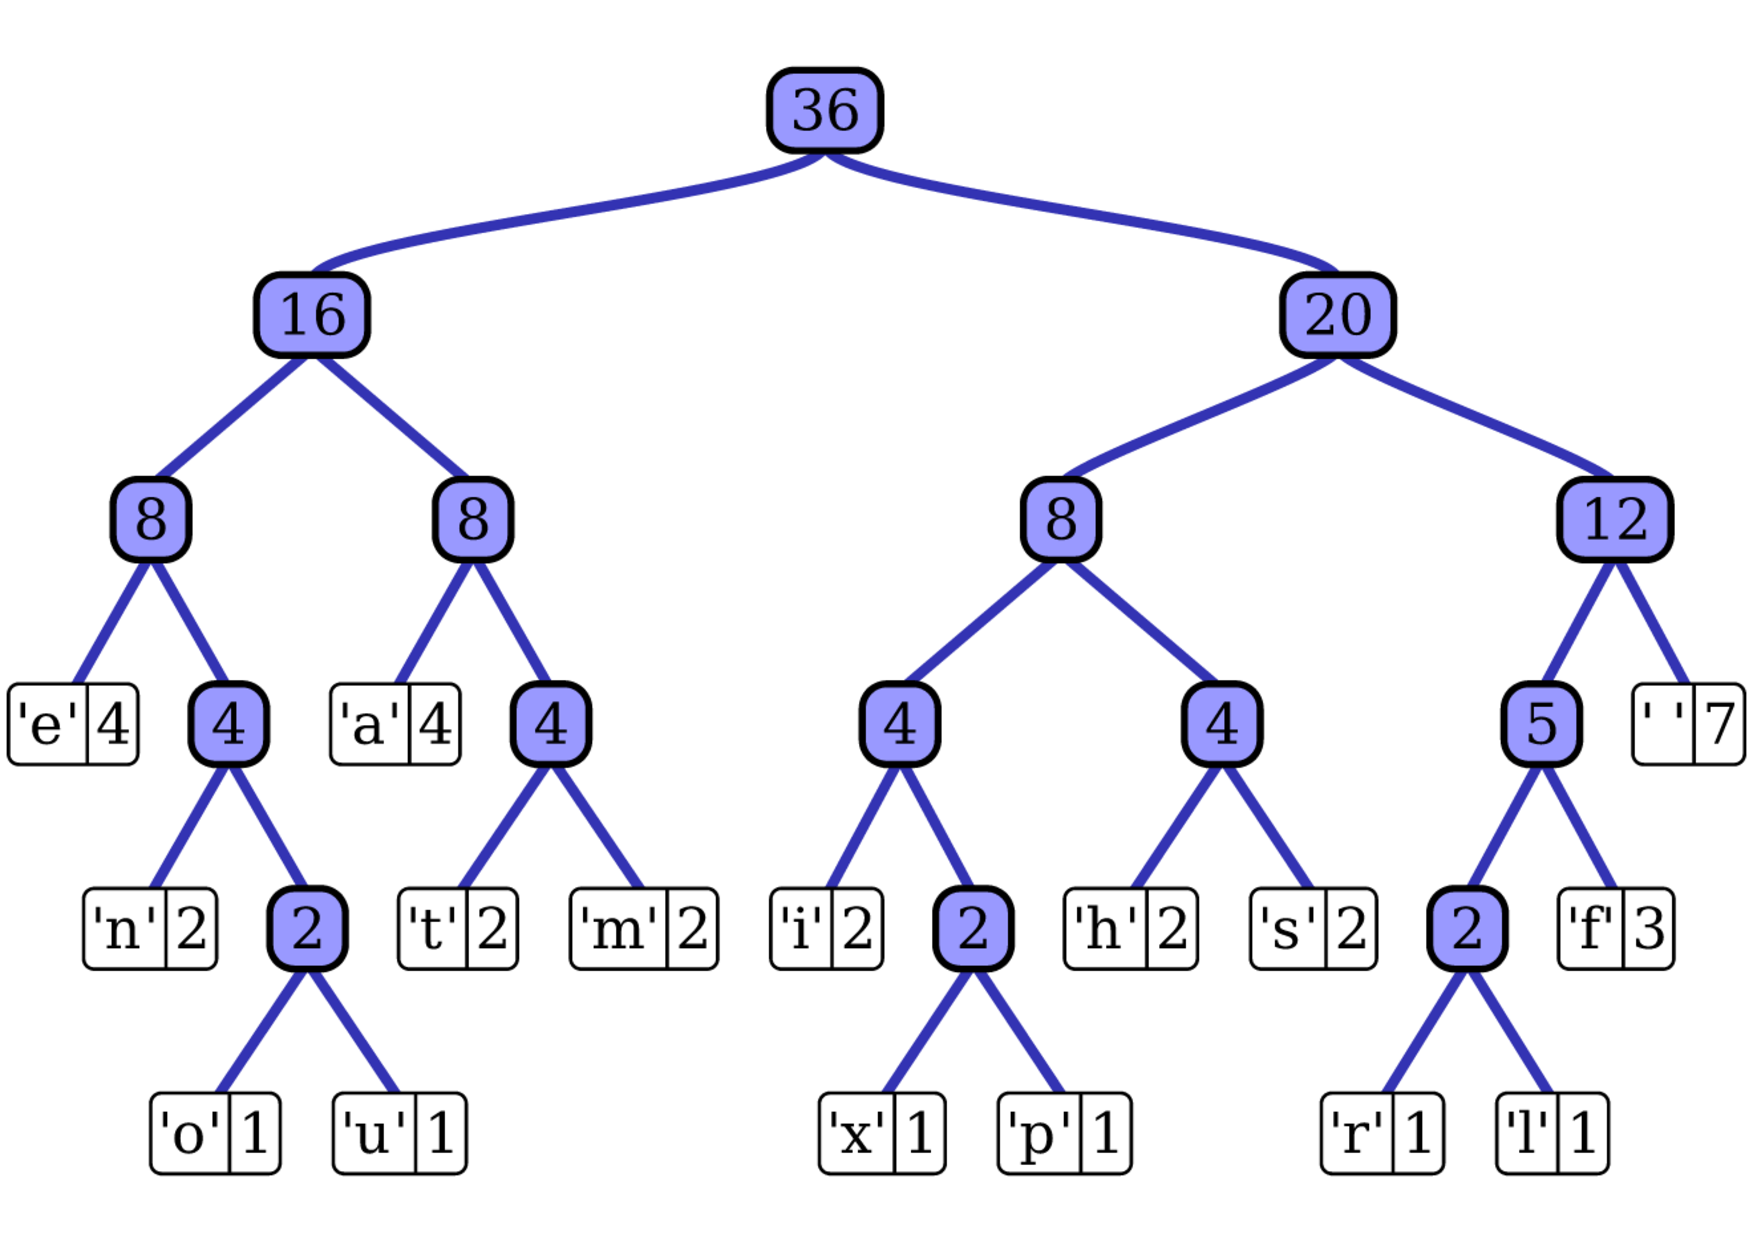
\includegraphics[width=8cm]{huffman}}{8cm}
	 			
	 \ \\			
	 L'arbre que l'on obtient n'est pas unique car parfois on opère un choix parmi plusieurs regroupements valides.\\
	
	 Voici dans les grandes lignes comment l'arbre ci-dessus a été crée :
	 On crée une variable \tw{poids} qui prendra tout au long de l'algorithme le minimum des poids des feuilles , des n\oe uds construits (parmi les 
	 feuilles se trouvent les lettres non encore placées dans l'arbre).
	\begin{enumerate}[--]
	\item 	Le poids minimal est 1 : \tw{poids=1}.
	\item 	On met o et u ensemble : poids 2, de même pour x et p et r et l 
			(on aurait très bien pu mettre o avec x et p avec u).
	\item 	On a epuisé les  feuilles de poids 1, \tw{poids=2} donc on peut regrouper des n\oe uds de poids 2, ou bien ajouter des feuilles de poids 
	2 entre elles, ou bien mélanger.\\
			
	\item 	On arrive à 'f', \tw{poids=3}. On le met avec un n\oe ud ou une lettre de poids 2, on obtient alors un n\oe ud de poids 5, mais attention : 
	\tw{poids=4}.
	\item 	Puisque \tw{poids=4}, on regroupe les n\oe uds et les lettres de poids 4, puis \tw{poids=5} et on n'a plus le choix : le n\oe ud de poids 
	5 va avec l'espace (pour créer un n\oe ud de poids 12), \tw{poids=8}, on assemble, \tw{poids=12} etc.
\end{enumerate}		 
	 
	 Ainsi la lettre 'u' (qui n'apparaît qu'une fois) est codée 11000. L'espace est, elle, codée 000.\\
	 Plus un caractère est fréquent, plus il figure haut dans l'arbre, et plus son codage est court.\\
	 
\begin{exercice}
 Quelle est, en bits, la taille de \og this is an example of a huffman tree\fg{} une fois le codage effectué ?\\

	 Puisque dans cette phrase, tous les caractères sont dans la table ANSI (7 bits par caractère), quel est le taux de compression ? \\ %1 - 135 / 
	 %36*7 presque 46
\end{exercice}
 
 
 \begin{exercice}[ : Projet Huffman]
 Créer un programme qui compresse des fichiers texte à l'aide de la méthode de Huffman.
 \end{exercice}
\section{Programmation - distance de similarité}
 
\subsection{En théorie}
 \double{
 	Compresser une information, cela revient \textit{grosso modo} à éliminer les redondances qu'elle comporte.\\
	En partant de cette idée, on considère deux informations A et B représentées par au moins un bit (non nulles). 
	Notons c un algorithme de compression performant (gzip par exemple) et AB le concaténé de A et de B (c'est-à-dire A et B \og mis à la suite\fg).\\
	Supposons que A et B aient un contenu commun (en noir) alors lorsqu'on compresse AB, ce contenu commun n'est compté qu'une fois, de sorte que 
	$$c(A)+c(B)-c(AB)$$
	est une bonne estimation de ce contenu commun.
 }
{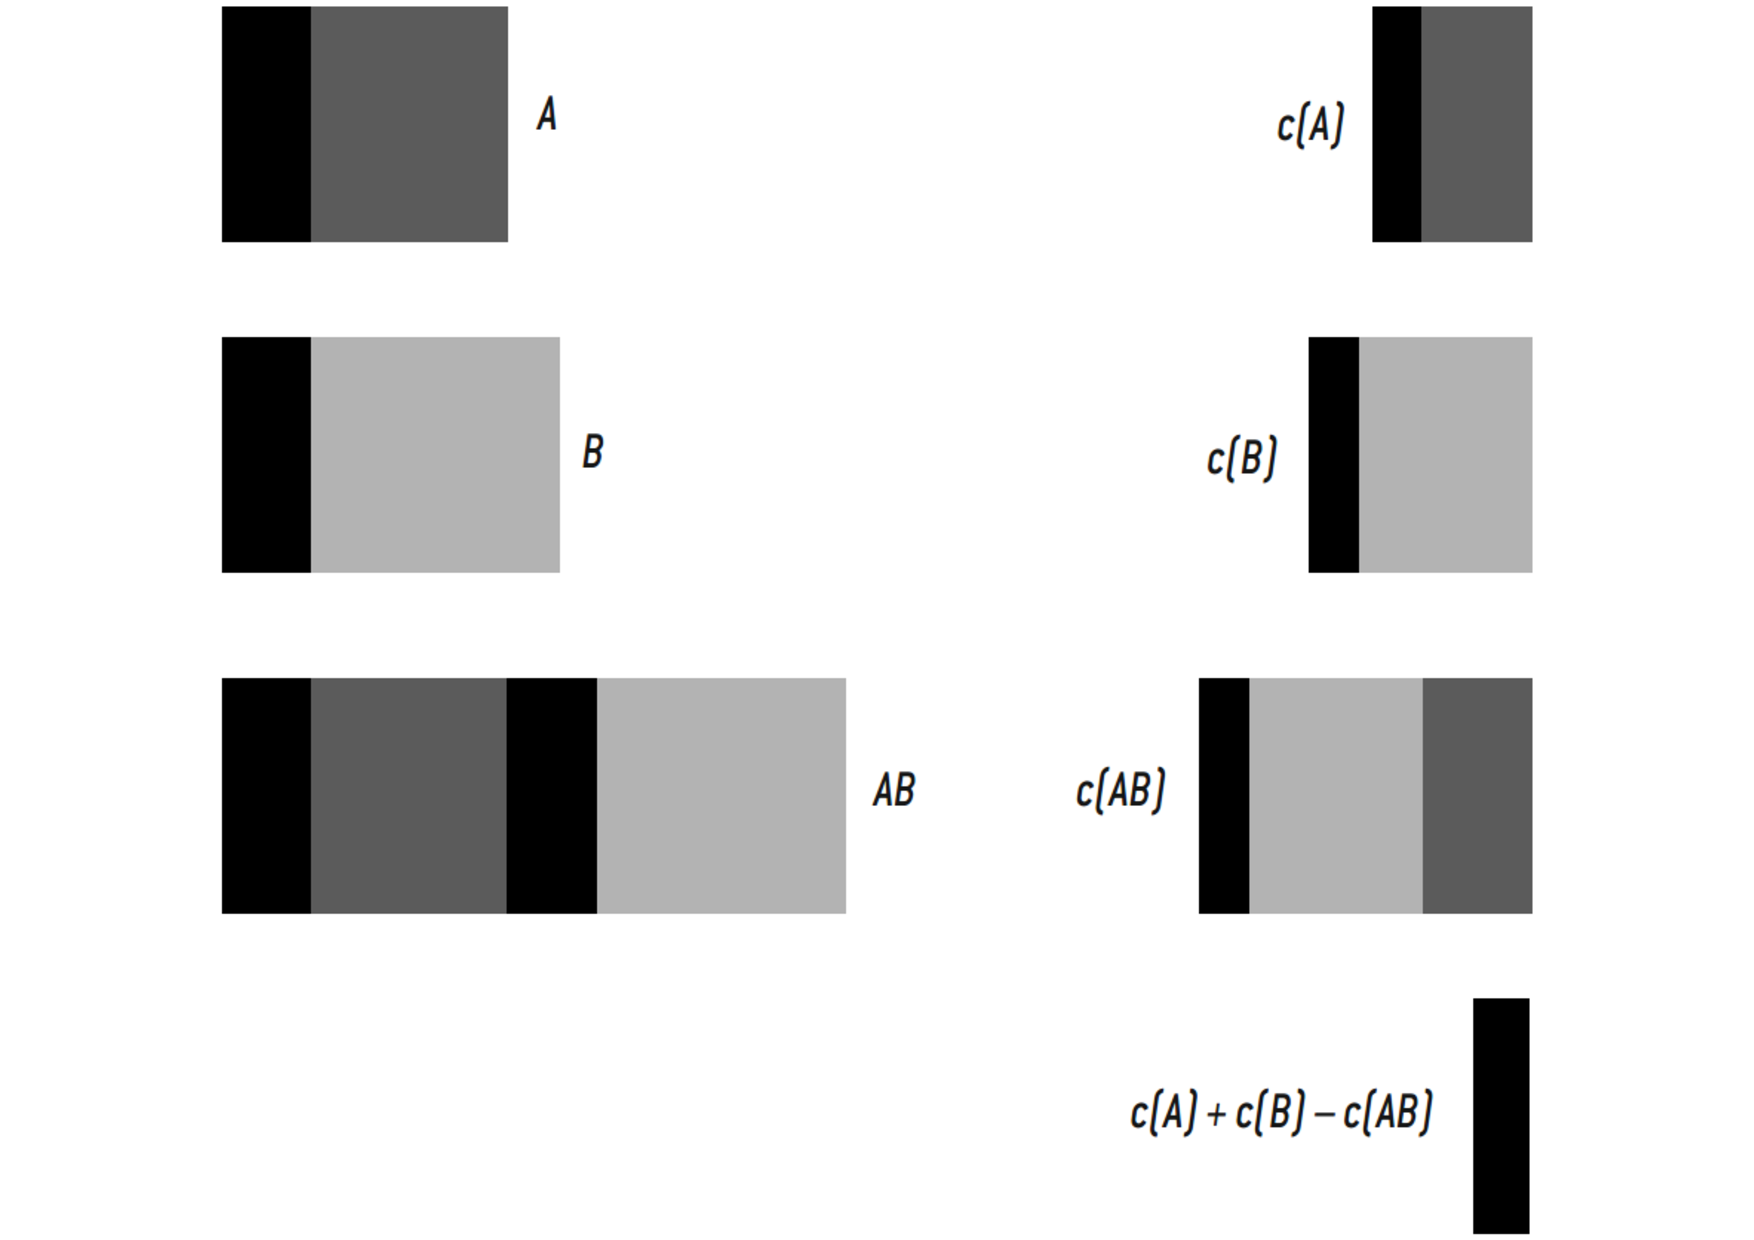
\includegraphics[width=7cm]{distance}}{7cm} 
\ \\

On définit la \textbf{distance de similarité entre A et B} par $$d(A,B)=1-\dfrac{c(A)+c(B)-c(AB)}{ \max\left(c(A),c(B)\right)}$$

En théorie, ce que l'on vient de définir est une \textbf{distance} : quelles que soient les informations \og non nulles\fg{}  A, B, et C on a :
\begin{enumerate}[--]
	\item 	$d(A,B)\geq 0$ 
	\item 	$d(A,B)=0$ si et seulement si $A=B$.
	\item 	$d(A,B)=d(B,A)$\hspace*{6em}(symétrie)
	\item 	$d(A,C)\leqslant d(A,B)+d(B,C)$ \hspace*{2em}(inégalité triangulaire)
\end{enumerate}

\subsection{Intérêts}

	\double{
			On peut se servir de la distance de similarité pour classer des informations de même nature suivant leur ressemblance.\\
			
			On a évalué ici les distances séparant 19 romans russes suivant la méthode précédente, puis on les a triés en rassemblant les plus 
			proches. On a obtenu le diagramme ci-contre.\\
			Seul un roman de Tolstoï est mal classé.\\
			
			Cette méthode est aussi appliquée en génétique : c'est l'ADN des différentes espèces que l'on compare, puis on établit un classement des 
			espèces.}{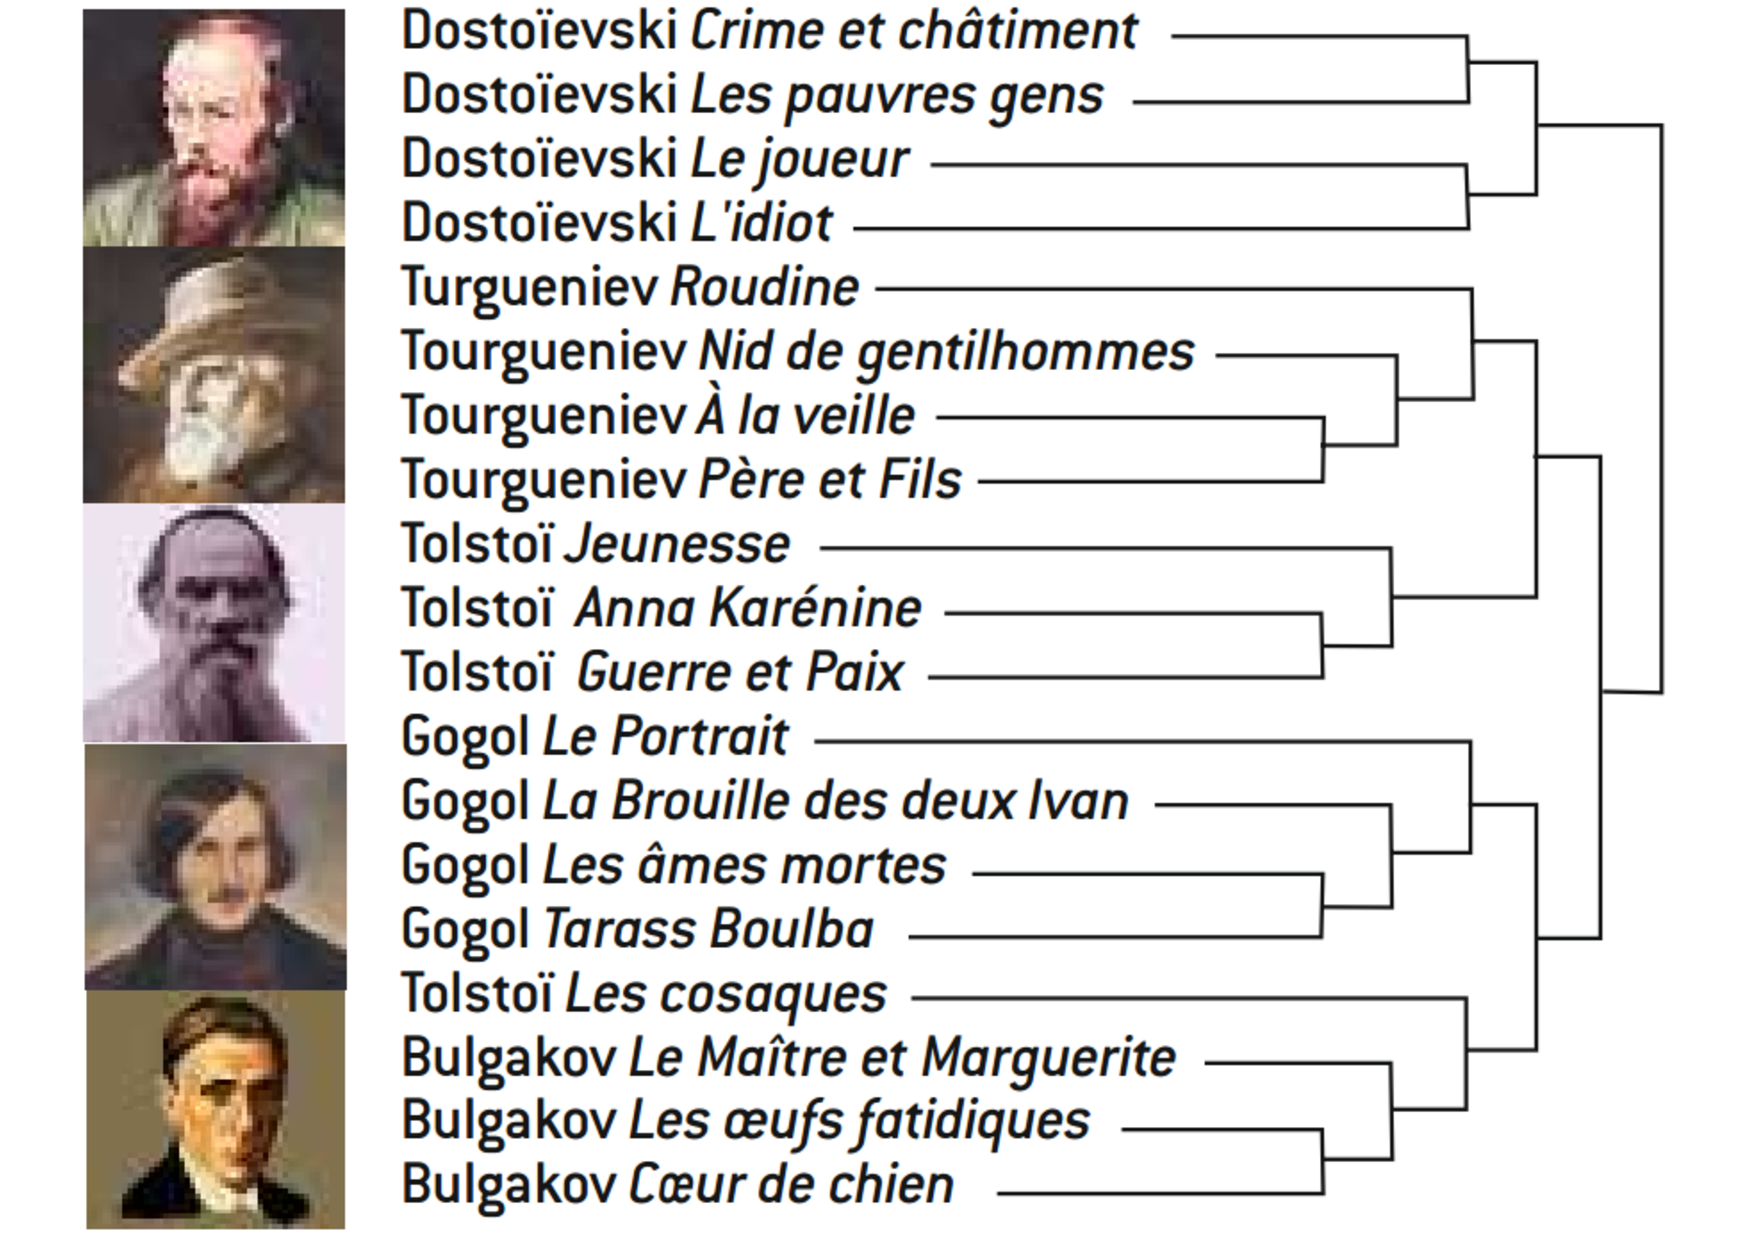
\includegraphics[width=8cm]{livres}}{8cm}



\begin{exercice}
Nous allons étudier les distances séparant quelques langues à partir de fichiers texte : il s'agit de la Déclaration Universelle des Droits de 
l'Homme, traduite en diverses langues.\\
Vous allez travailler sur le fichier \texttt{classement\_langues.py}.\\
Dans celui-ci, est déjà présente la fonction \pythoninline{taille_compressee} dont vous vous servirez.\\

\textbf{1.} Commencer par coder la fonction \pythoninline{distance}, qui donne la distance entre 2 fichiers.\\

\textbf{2.} Que vaut \pythoninline{distance('anglais','anglais')} ?\\
 Que peut-on en déduire par rapport à la théorie ?\\



\textbf{3.} Comparer \pythoninline{distance('anglais','francais')} et  \pythoninline{distance('francais','anglais')}.\\
Proposer une modification de la fonction \tw{distance} pour qu'elle soit symétrique.\\



\textbf{4.} Coder la fonction \pythoninline{calcule_distances} qui, à partir d'une liste de fichiers, calcule les distances les séparant les uns des autres 
(attention : ne pas faire de calculs inutiles).\\

\textbf{5.} Exécuter \\

\mintinline[fontsize=\footnotesize]{python}{calcule_distances(['francais','portuguais','espagnol','tcheque',slovaque'])}

Commenter les résultats.\\

\end{exercice}
\end{document}
